\documentclass{wilson-report}

% ── PDF Metadata ──
\hypersetup{
  pdftitle={The US Economic Outlook: Navigating the Tariff Fog},
  pdfsubject={Macro / Economic Analysis},
  pdfkeywords={US Economy, GDP, Inflation, Federal Reserve, Tariffs, 2026 Outlook}
}

\begin{document}

% ── TITLE PAGE ──
\maketitlepage
  {The US Economic Outlook:\\ Navigating the Tariff Fog}
  {Macro / Economic Analysis}
  {US Economy, Fixed Income, Equities}
  {Strategic (12-month)}

% ── EXECUTIVE SUMMARY ──
\execsummary{
\begin{itemize}[leftmargin=1.2em, itemsep=4pt]
  \item \textbf{The View:} US economy grinding towards below-trend growth of 1.5--2.0\% over the next 12 months, with elevated but not catastrophic recession risk (30--40\%). \neutralweight{} on US growth assets, \conviction{M} conviction, 12-month strategic horizon.
  \item \textbf{The Evidence:} Q4 2025 GDP decelerated to 1.4\% annualised (BEA, 20 Feb 2026); core PCE inflation stuck at 3.0\% (BEA, Dec 2025); the Fed is boxed in between sticky inflation and slowing growth --- a ``stagflation-lite'' trap.
  \item \textbf{The Risk:} The SCOTUS tariff ruling (20 Feb 2026) has reshuffled trade policy --- Trump's pivot to a 10\% Section 122 surcharge and the \$175bn refund overhang create a fiscal/trade wildcard that could break in either direction.
  \item \textbf{The Expression:} Favour duration in the belly of the curve (5Y UST); underweight cyclical equities vs.\ defensive quality; hedge tail risk via long gold and USD/JPY puts. Avoid outright equity shorts --- the two-speed economy means the top decile of consumers and AI capex can sustain growth longer than bears expect.
\end{itemize}
\textit{All market data as of close 21 February 2026.}
}

% ══════════════════════════════════════════════════════════════
\section{Macro Context}
% ══════════════════════════════════════════════════════════════

The US economy enters 2026 in an unusual and internally contradictory state. On the surface, the expansion continues --- real GDP grew 2.8\% in 2024 and an estimated 2.5\% in 2025 on a Q4/Q4 basis (BEA). But the composition and trajectory tell a more nuanced story.

\subsection{Growth: Decelerating, Not Collapsing}

Q4 2025 GDP came in at just 1.4\% annualised (BEA, advance estimate, 20 Feb 2026), a sharp deceleration from the 4.4\% print in Q3. The slowdown was broad-based: consumer spending growth moderated, business fixed investment was flat, and net exports were a drag as importers front-loaded purchases ahead of expected tariff increases. Government spending also decelerated as DOGE-driven federal workforce cuts --- approximately 271,000 positions eliminated in 2025, a 9\% reduction in federal employment (OPM via Cato Institute, Jan 2026) --- began to weigh on outlays, though total federal spending still rose by \$248bn YoY through November 2025 due to entitlement autopilot.

\begin{figure}[H]
  \centering
  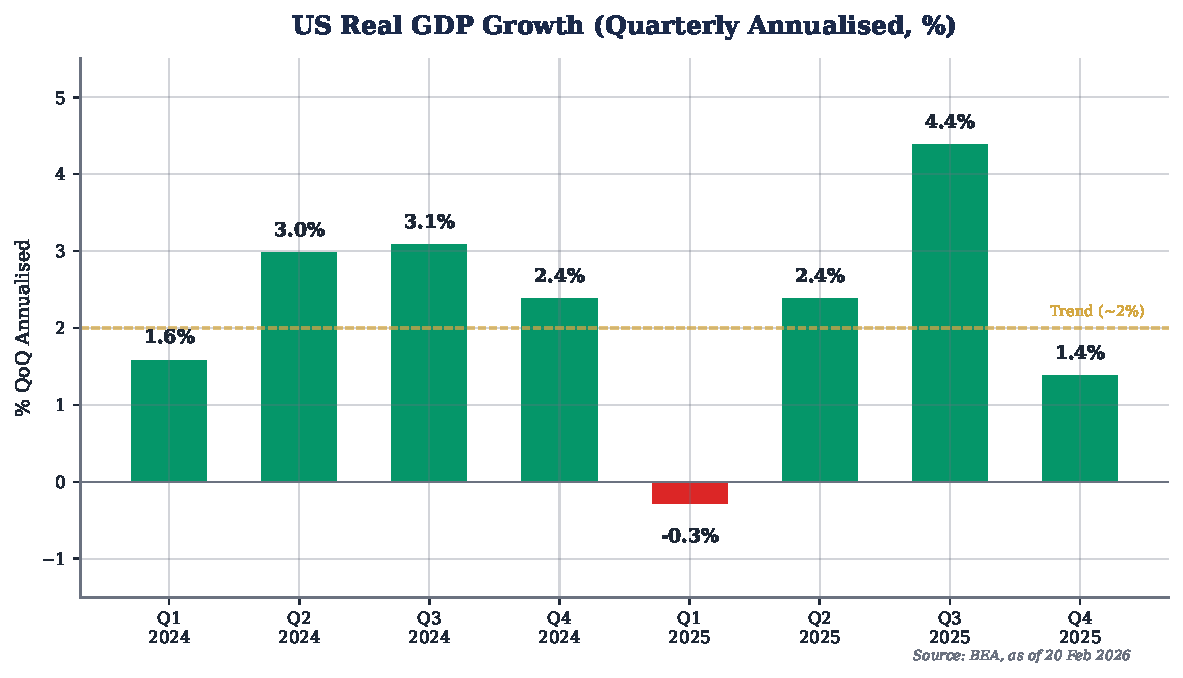
\includegraphics[width=0.95\textwidth]{chart_gdp_growth.pdf}
  \caption{US Real GDP Growth --- quarterly annualised rate. The Q1 2025 contraction (-0.3\%) was largely tariff-distorted (import front-loading). Q4 2025 deceleration to 1.4\% is more concerning as a genuine demand signal. Source: BEA, as of 20 Feb 2026.}
\end{figure}

The ISM Manufacturing PMI surged to 52.6 in January 2026 --- its highest since August 2022 and the first expansion reading in 12 months (ISM, 1 Feb 2026). New orders jumped to 57.1 from 47.4. However, the ISM chair cautioned that January is a seasonal reorder month and that ``some buying appears to be to get ahead of expected price increases due to ongoing tariff issues.'' The S\&P Global flash Manufacturing PMI for February already moderated to 51.2, the weakest in seven months (S\&P Global, 21 Feb 2026). This pattern --- a sharp PMI bounce followed by rapid fade --- is consistent with tariff-pull-forward dynamics rather than a genuine manufacturing recovery.

\keyinsight{The US economy is exhibiting a ``two-speed'' dynamic: the top 10\% of consumers (buoyed by \$70tn in household equity wealth and AI-driven corporate spending) account for nearly half of all consumer spending, while the bottom half is ``already in recession to some extent'' (Deloitte, Feb 2026). This bifurcation makes aggregate data misleading --- headline GDP masks genuine stress in the broad economy.}

\subsection{Inflation: Sticky, Not Re-Accelerating}

Inflation remains the binding constraint on policy. CPI fell to 2.4\% YoY in January 2026 (BLS), but core PCE --- the Fed's preferred gauge --- printed at 3.0\% YoY in December 2025 (BEA), well above the 2\% target and re-accelerating from the 2.6\% trough reached in mid-2025. The divergence between headline CPI (pulled down by energy) and core PCE (sticky services, shelter, and insurance costs) is a key feature of the current environment.

\begin{figure}[H]
  \centering
  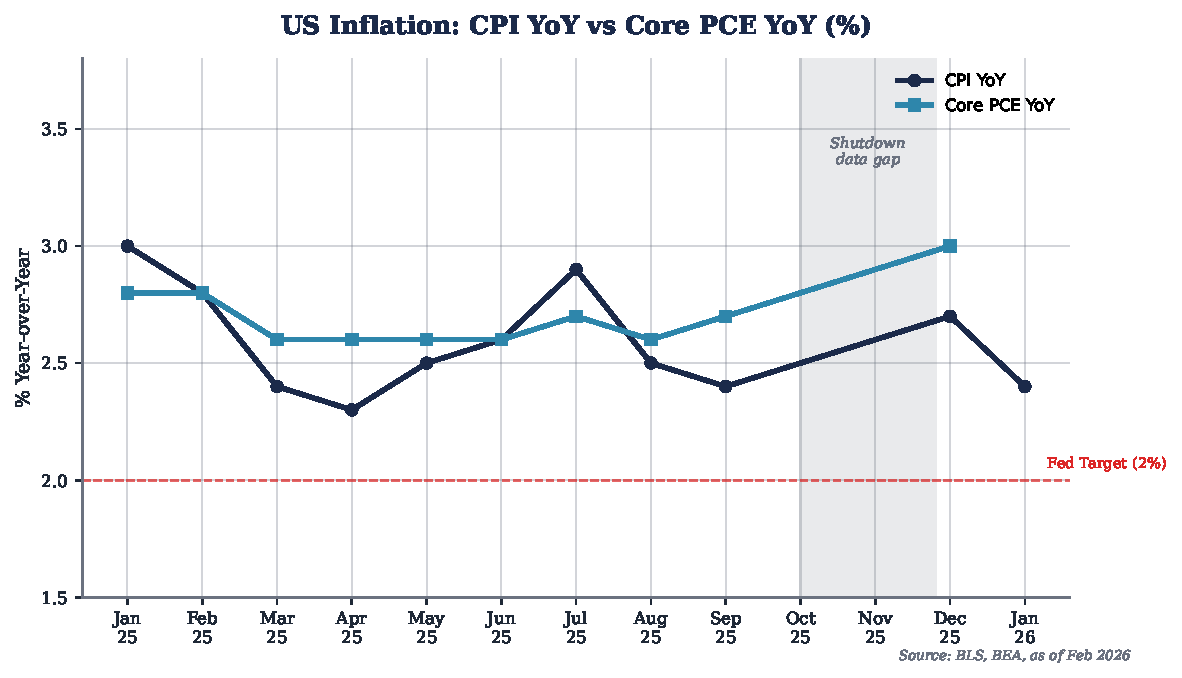
\includegraphics[width=0.95\textwidth]{chart_inflation.pdf}
  \caption{US Inflation --- CPI YoY vs Core PCE YoY. The government shutdown in late 2025 created a data gap (shaded). Core PCE's re-acceleration to 3.0\% in December is the critical constraint on Fed easing. Source: BLS, BEA, as of Feb 2026.}
\end{figure}

Tariff pass-through is the key upside risk to inflation. The SCOTUS ruling on 20 February struck down IEEPA-based tariffs, but the administration immediately imposed a 10\% Section 122 surcharge effective 24 February. Section 301 tariffs on China remain in force. The net tariff regime has been partially reduced but remains substantial --- and the uncertainty itself is a cost, as firms cannot plan pricing or sourcing with confidence.

\textbf{So what?} The inflation picture argues against aggressive Fed easing, keeps real yields elevated, and favours assets with pricing power. The ``last mile'' of disinflation is proving stubbornly difficult, and tariff noise adds a structural floor under goods prices.

\subsection{Federal Reserve: Boxed In}

The Fed has cut the federal funds rate by 175bps since September 2024, from 5.50\% to the current 3.625\% (upper bound of 3.50--3.75\% target range). But the pace has stalled --- the last cut was in September 2025, and the Fed has been on hold for five months.

\begin{figure}[H]
  \centering
  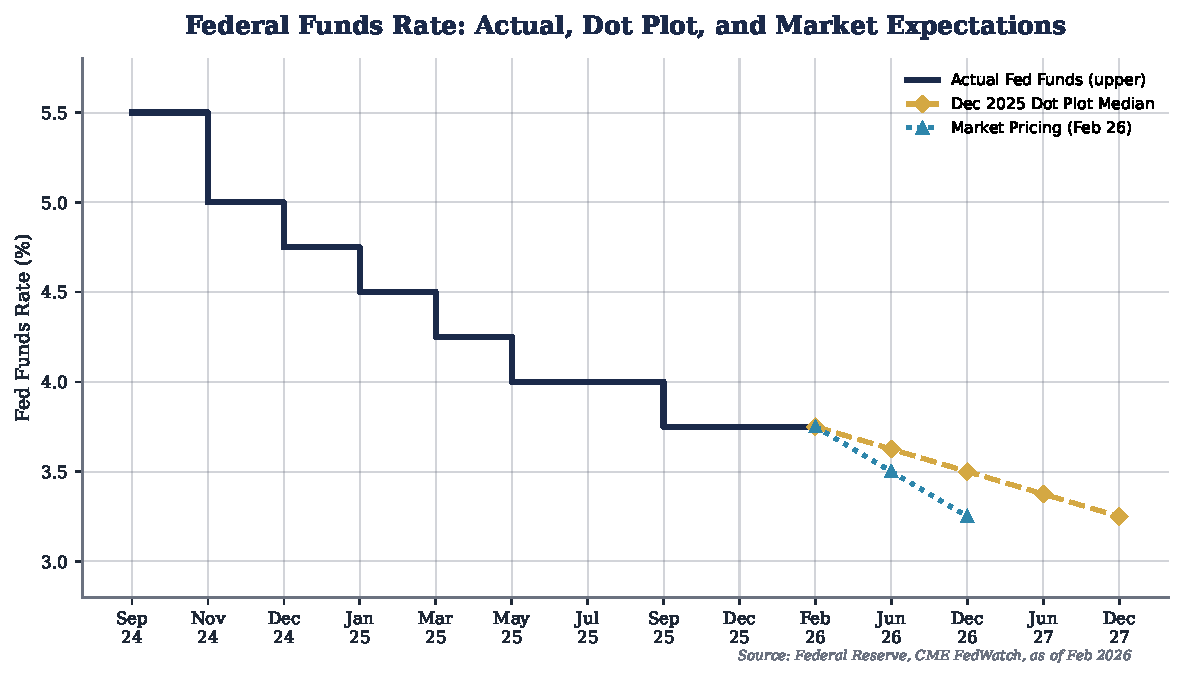
\includegraphics[width=0.95\textwidth]{chart_fed_rate.pdf}
  \caption{Fed Funds Rate: actual path vs December 2025 dot plot median vs current market pricing. Markets price approximately two 25bp cuts by year-end (to 3.25\%), roughly in line with the dot plot. Source: Federal Reserve, CME FedWatch, as of Feb 2026.}
\end{figure}

The January FOMC minutes revealed a divided committee. With core PCE at 3.0\%, several governors pushed back against further easing until inflation shows ``sustained progress'' back toward 2\%. Meanwhile, the labour market is softening --- unemployment edged to 4.3\% in January 2026, the highest in over four years (BLS) --- creating a classic dual-mandate tension.

Markets currently price approximately two 25bp cuts by December 2026, bringing the rate to 3.25\%. The December 2025 dot plot median pointed to a similar trajectory. This pricing seems reasonable as a base case, but the range of outcomes is wide: a genuine growth scare would force faster cuts, while a tariff-driven inflation spike could delay them entirely.

\textbf{So what?} The Fed is in ``wait and see'' mode. This is a neutral-to-negative backdrop for risk assets --- it removes the tailwind of a proactive easing cycle while leaving the economy exposed to shocks without a pre-committed policy put.

% ══════════════════════════════════════════════════════════════
\section{Core Analysis}
% ══════════════════════════════════════════════════════════════

\subsection{The Tariff Regime: SCOTUS Ruling and the Pivot}

The Supreme Court's 6--3 decision in \textit{Learning Resources, Inc. v.\ Trump} (20 Feb 2026) struck down all IEEPA-based tariffs, ruling that IEEPA does not grant the President authority to impose tariffs (SCOTUSblog, 20 Feb 2026). This was the single most significant trade policy development of the cycle.

\textbf{What was struck down:} 25\% tariffs on Canadian and Mexican imports, 10\% fentanyl-related tariffs on China, and the ``reciprocal'' tariffs of 10--50\% on all trading partners. IEEPA tariffs accounted for roughly half of all import tax revenue being collected (Penn Wharton Budget Model, 20 Feb 2026).

\textbf{What remains:} Section 301 tariffs on China (the bulk of the China tariff architecture), Section 232 tariffs on steel and aluminium, and a new 10\% ``temporary import surcharge'' under Section 122 of the Trade Act of 1974, imposed by executive order on the same day for 150 days.

\textbf{The refund overhang:} Importers have paid an estimated \$175--200bn+ in IEEPA tariff duties since 2025 (CNBC, Penn Wharton, 20 Feb 2026). The Court did not address refunds, leaving this to the Court of International Trade. This creates a material fiscal/cash flow wildcard: if refunds are ordered, they represent a one-off boost to corporate cash flows and could be deflationary; if denied or delayed, the status quo persists.

\textbf{The legislative angle:} It is unlikely that Congress will extend new tariff authority in 2026 with midterm elections approaching (CFR, Feb 2026). The Section 122 surcharge has a 150-day statutory limit and caps at 15\%, significantly constraining the administration's tariff ceiling relative to the IEEPA regime.

\textbf{So what?} The net effect is a \textit{reduction} in tariff uncertainty, but not its elimination. The effective tariff rate on US imports has declined --- particularly on Canadian and Mexican goods --- which is mildly positive for growth and mildly disinflationary. But the administration's willingness to immediately pivot to alternative legal authorities signals that trade friction remains a structural feature. Companies face a lower but still-elevated tariff floor with continued legal and policy uncertainty.

\subsection{Labour Market: Cooling, Not Crashing}

The labour market is the key variable to watch for recession timing. Unemployment rose to 4.3\% in January 2026 (BLS), the highest in four years. Wage gains are slowing, hiring has ``largely flatlined since the summer of 2025'' (Yahoo Finance / Bankrate, Feb 2026), and initial claims have drifted higher.

The DOGE-driven federal workforce reduction (271,000 positions) has had a direct impact: former federal workers are struggling to find equivalent roles, and the IRS --- which shed over 26,000 employees --- faces capacity constraints that may reduce tax compliance revenue by \$323bn over the next decade (Yale Budget Lab, Feb 2026). The ripple effects through government contractors and federal-employment-dependent regional economies (Washington DC metro, military towns) are underappreciated.

However, the labour market is not in freefall. Private sector hiring continues, albeit at a subdued pace. The two-speed dynamic means that tech, AI, and professional services continue to add roles while retail, government, and lower-skilled sectors face headwinds.

\textbf{So what?} The labour market is consistent with a late-cycle deceleration rather than an imminent recession. The unemployment rate is a lagging indicator, but the direction of travel is unambiguously weaker. If unemployment breaches 4.5\% and claims accelerate, recession risk escalates sharply.

\subsection{Fiscal Policy: The DOGE Paradox}

DOGE set out to cut \$2 trillion in federal spending. That target was progressively reduced to \$1 trillion, then \$150 billion. The reality: federal spending \textit{rose} by \$248bn through November 2025 vs the prior year (Cato Institute, Feb 2026). Why? Because 75\% of federal spending is mandatory (Social Security, Medicare, Medicaid, interest) and is on autopilot. DOGE succeeded in cutting the workforce but failed to cut spending.

Meanwhile, the costs of disruption are mounting. The nonpartisan National Priorities Project estimated DOGE actions will cost \$135bn in FY2026 through paid leave, re-hiring, productivity loss, and revenue foregone (CBS News, Feb 2026). The IRS predicts over \$500bn in lost revenue over a decade from reduced enforcement capacity.

The fiscal deficit remains wide at approximately 6.5\% of GDP. With the 2017 Tax Cuts and Jobs Act provisions set to expire at the end of 2025, the legislative fight over extension adds another layer of fiscal uncertainty. If extended (likely given Republican congressional majorities), the deficit widens further, supporting nominal growth in the near term but adding to the term premium and long-end yield pressure.

\textbf{So what?} Fiscal policy is inadvertently expansionary despite the efficiency rhetoric. The wide deficit supports demand but pressures long-end rates. The DOGE disruption to government services (IRS, Social Security, USAID) creates micro-level drag that won't show up in GDP but will erode institutional capacity and public confidence.

\subsection{Financial Conditions and Credit}

Financial conditions remain relatively accommodative despite the Fed pause. The 10-year Treasury yield at 4.08\% (21 Feb 2026) is well below the 5.0\% peak reached in 2025. The HY OAS (ICE BofA) sits at approximately 286bps --- tight by historical standards, suggesting limited credit stress. Equity markets near all-time highs support the wealth effect.

However, the term premium on the 10-year at 0.59\% (Kim-Wright model, Jan 2026) is at its highest in a decade, reflecting fiscal concerns, inflation uncertainty, and tariff risk. The yield curve is positively sloped (2s10s spread ~60bps), which removes the inversion recession signal but reflects the market pricing in persistent inflation risk rather than signalling healthy growth expectations.

\textbf{So what?} Financial conditions are a pillar of support for the ``no recession'' base case. HY spreads at 286bps imply default expectations well below recession levels. The key risk is a sudden tightening --- either from a policy shock, a credit event, or a sharp equity correction that triggers the wealth-effect feedback loop (a 10\% equity drawdown would erase ~\$7tn in household wealth).

\begin{figure}[H]
  \centering
  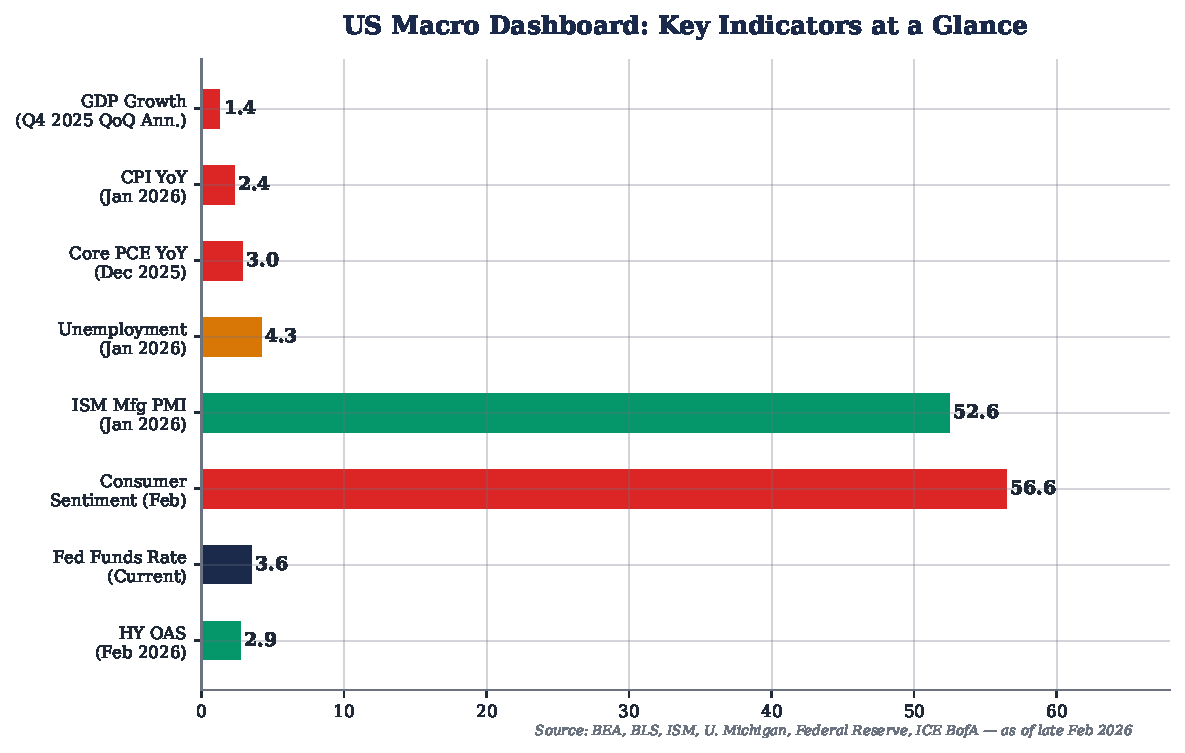
\includegraphics[width=0.95\textwidth]{chart_dashboard.pdf}
  \caption{US Macro Dashboard. Green = supportive; red = concerning; amber = mixed. Core PCE at 3.0\% and consumer sentiment at 56.6 (U. Michigan, Feb 2026, preliminary) are the standout negatives. Source: Various, as of late Feb 2026.}
\end{figure}

\subsection{Consumer Sentiment: The Confidence Gap}

The University of Michigan consumer sentiment index fell to 56.6 in the preliminary February 2026 reading --- well below the long-run average of ~84 and consistent with the ``two-speed'' thesis. Consumers expect higher prices (tariff anxiety) and are less confident about income prospects. This creates a tension: soft data (sentiment) is much weaker than hard data (actual spending, GDP). Historically, soft data eventually pulls hard data lower --- but the lag can be long, and the wealthy consumer segment is less sentiment-sensitive.

\textbf{So what?} Sentiment at these levels is a yellow flag, not a red one. It argues for caution on consumer discretionary exposure and supports the quality/defensive tilt in equities.

% ══════════════════════════════════════════════════════════════
\section{Scenario Analysis}
% ══════════════════════════════════════════════════════════════

\begin{tabularx}{\textwidth}{>{\bfseries\raggedright\arraybackslash}m{1.3cm} >{\centering\arraybackslash}m{1cm} X >{\raggedright\arraybackslash}m{2cm} >{\raggedright\arraybackslash}m{3cm}}
\toprule
\rowcolor{BrandNavy} \color{white}\textbf{Scenario} & \color{white}\textbf{Prob.} & \color{white}\textbf{Description} & \color{white}\textbf{GDP Growth} & \color{white}\textbf{Key Driver} \\
\midrule
\bullrow Bull & 20\% & SCOTUS ruling triggers genuine tariff de-escalation; Section 122 surcharge expires without renewal; refunds boost corporate cash flow; Fed cuts 3--4 times. Inflation falls below 2.5\%. Consumer confidence recovers. & 2.5--3.0\% & Tariff removal + Fed easing + refund stimulus \\
\baserow Base & 50\% & Tariff uncertainty persists at lower levels; Fed delivers 1--2 cuts; inflation grinds slowly toward 2.5\% but doesn't reach target. Growth slows to below-trend 1.5--2.0\%. Labour market softens further but no mass layoffs. & 1.5--2.0\% & Muddle-through; sticky inflation caps Fed; two-speed economy sustains \\
\bearrow Bear & 30\% & Tariff escalation via Section 301 expansion or new legislation; inflation re-accelerates above 3.5\%; Fed unable to cut; equity correction triggers wealth-effect feedback; unemployment breaches 5.0\%. Recession by Q4 2026. & 0.0 to -1.0\% & Stagflation trap; policy error; consumer capitulation \\
\bottomrule
\end{tabularx}

\vspace{0.5em}
\textit{Probability-weighted expected GDP growth: $(0.20 \times 2.75) + (0.50 \times 1.75) + (0.30 \times -0.5) = 1.28\%$.} This is below the consensus estimate of ~2.0\% (Bloomberg survey), reflecting our heavier bear-case weight driven by tariff and inflation risks.

% ══════════════════════════════════════════════════════════════
\section{Cross-Asset Implications}
% ══════════════════════════════════════════════════════════════

\textbf{Equities:} Below-trend growth with sticky inflation is not a hospitable environment for broad equity beta. The S\&P 500 forward P/E of ~23.6x (Investing.com, Feb 2026) prices in a continuation of the AI-driven earnings cycle with no macro disruption. Favour quality/defensive over cyclical. The ``two-speed'' economy means mega-cap tech with pricing power and AI capex exposure can outperform while the median stock struggles. This is \textit{not} the environment for a great rotation into small caps, despite their valuation discount.

\textbf{Fixed Income:} The belly of the curve (5Y) offers the best risk-adjusted carry. The Fed is likely to resume cutting in H2 2026, which supports front-end and intermediate maturities. Long-end remains vulnerable to term premium expansion from fiscal deficits and tariff-driven inflation risk. Favour 5Y UST over 10Y+.

\textbf{Credit:} HY spreads at 286bps are tight and offer limited compensation for downside scenarios. If recession probability is genuinely 30\%, HY is mispriced. Favour IG over HY; within HY, favour secured/short-duration.

\textbf{FX:} The dollar faces cross-currents. Tariff reduction is dollar-negative (less safe-haven demand, reduced trade surplus recycling); rate differentials remain dollar-supportive vs.\ EUR and JPY. Net: range-bound DXY, but biased lower over 12 months as the Fed resumes cutting and fiscal concerns weigh.

\textbf{Gold:} The stagflation-lite backdrop, fiscal concerns, and geopolitical uncertainty all support gold. It serves as the optimal portfolio hedge in an environment where bonds and equities may correlate positively (as they do when inflation is the dominant risk).

% ══════════════════════════════════════════════════════════════
\section{Risks to the View}
% ══════════════════════════════════════════════════════════════

\begin{itemize}[leftmargin=1.2em, itemsep=4pt]
  \item \textbf{AI capex sustains the cycle longer than expected.} If the AI investment boom continues to drive corporate spending, productivity gains, and tech earnings growth, the US can grow above trend despite headwinds. Deutsche Bank has noted that ``the US economy might already be close to a recession if not for tech spending'' (Bankrate, Feb 2026). If AI capex accelerates, the bull case becomes more probable.
  \item \textbf{Tariff de-escalation surprises to the upside.} The SCOTUS ruling may force a genuine policy pivot if alternative legal authorities prove insufficient. Congressional pressure ahead of midterms could push the administration toward negotiated trade deals. This would be unambiguously positive for growth and disinflationary.
  \item \textbf{Consumer capitulates faster than expected.} The wealth-effect feedback loop is the key tail risk. The top 10\% of consumers are propping up the economy, but they are also the most equity-sensitive. A sustained 10\% equity decline could erase ~\$7tn in household wealth, reducing aggregate demand by an estimated \$280bn (Investing.com, Feb 2026). This is the path to a faster, deeper recession than our base case envisions.
  \item \textbf{Tariff refund overhang creates a fiscal shock.} If courts order \$175bn+ in IEEPA tariff refunds, this is a material cash flow event. The fiscal impact (widening the deficit) and the corporate impact (one-off cash boost to importers) are hard to model and could break in either direction.
  \item \textbf{IRS revenue shortfall is worse than expected.} The Yale Budget Lab's estimate of \$323bn in lost tax revenue over a decade from DOGE-driven IRS cuts could prove conservative. If tax compliance deteriorates sharply, the deficit blows out further, adding to long-end yield pressure and crowding out private investment.
\end{itemize}

The steelmanned bull case: The US economy has repeatedly defied recession predictions since 2022. The labour market, while cooling, is not breaking. AI capex is a genuine productivity catalyst with historical precedent (1990s tech boom sustained above-trend growth for a decade). The SCOTUS ruling may be the beginning of genuine tariff de-escalation, and the refund overhang could act as a one-off fiscal stimulus. Financial conditions remain loose. In this framing, the ``stagflation-lite'' narrative is overblown, and the economy reaccelerates in H2 2026 as tariff headwinds fade and the Fed resumes cutting. We give this 20\% probability --- not because the logic is wrong, but because it requires multiple things to go right simultaneously.

% ══════════════════════════════════════════════════════════════
\section{Key Indicators to Watch}
% ══════════════════════════════════════════════════════════════

\begin{tabularx}{\textwidth}{>{\raggedright\arraybackslash}m{2.2cm} >{\raggedright\arraybackslash}m{1.8cm} X X >{\raggedright\arraybackslash}m{2.2cm}}
\toprule
\rowcolor{BrandNavy} \color{white}\textbf{Indicator} & \color{white}\textbf{Current} & \color{white}\textbf{Confirming (Base)} & \color{white}\textbf{Disconfirming} & \color{white}\textbf{Next Trigger} \\
\midrule
ISM Mfg PMI & 52.6 (Jan) & Fades to 50--52 range in Feb/Mar, confirming pull-forward thesis & Sustains above 53 for 2+ months (bull); drops below 48 (bear) & 2 Mar 2026 \\
\midrule
Core PCE YoY & 3.0\% (Dec) & Gradual decline to 2.6--2.8\% by mid-2026 & Rises above 3.2\% (stagflation risk escalates; Fed cannot cut) & 28 Feb 2026 (Jan data) \\
\midrule
Unemployment Rate & 4.3\% (Jan) & Drifts to 4.3--4.5\% range; no acceleration in claims & Breaches 4.5\% with rising initial claims above 260K (recession signal) & 7 Mar 2026 (Feb NFP) \\
\midrule
HY OAS & ~286bps & Remains below 350bps; no credit stress & Blows out above 400bps (credit market pricing recession) & Continuous \\
\midrule
10Y UST Yield & 4.08\% & Drifts to 3.8--4.2\% range as Fed pauses & Rises above 4.5\% (term premium spike; fiscal concerns) or falls below 3.5\% (flight to safety) & Continuous \\
\midrule
Section 122 Tariff & 10\% surcharge & Maintained at 10\%; no escalation via other authorities & Increased toward 15\% cap or new Section 301 actions (inflation risk) & 24 Jul 2026 (150-day expiry) \\
\midrule
IEEPA Refund Ruling & Pending & Courts defer or phase refunds over 2+ years (limited macro impact) & Courts order lump-sum refund of \$175bn+ (fiscal shock) & CIT proceedings, Q2 2026 \\
\midrule
U. Michigan Sentiment & 56.6 (Feb prelim) & Stabilises above 55; no further deterioration & Falls below 50 (consumer capitulation; hard data likely to follow) & 28 Feb 2026 (final) \\
\bottomrule
\end{tabularx}

\textbf{Falsification criteria:} This below-trend-growth base case is falsified if (a) real GDP prints above 2.5\% annualised for two consecutive quarters in H1 2026 \textit{and} core PCE falls below 2.5\%, as this would indicate the economy is reaccelerating without an inflation constraint --- a clear bull scenario. Conversely, the ``no recession'' component is falsified if unemployment breaches 4.8\% and HY OAS exceeds 450bps simultaneously, which would indicate credit stress severe enough to warrant recessionary pricing.

% ══════════════════════════════════════════════════════════════
\section{Actionable Conclusions}
% ══════════════════════════════════════════════════════════════

\begin{itemize}[leftmargin=1.2em, itemsep=4pt]
  \item \textbf{Overall US growth view:} \neutralweight{} \conviction{M} --- Below-trend growth (1.5--2.0\%) with elevated but not dominant recession risk (30\%). Not bearish enough to position outright short, not bullish enough to chase beta.
  \item \textbf{Duration:} \overweight{} 5Y UST \conviction{M} --- The belly offers the best carry with optionality on both Fed cuts (bull) and flight-to-quality (bear). Avoid the long end (30Y) where term premium and fiscal supply risk dominate.
  \item \textbf{Equities:} \neutralweight{} broad S\&P 500 \conviction{M} --- Favour quality factor (high ROIC, low leverage, pricing power) over cyclical beta. \underweight{} consumer discretionary and small caps, which bear the brunt of the two-speed economy and tariff pass-through.
  \item \textbf{Credit:} \underweight{} HY \conviction{M} --- Spreads at 286bps do not compensate for 30\% recession probability. Favour short-duration IG.
  \item \textbf{Gold:} \overweight{} \conviction{H} --- The optimal hedge in a stagflation-lite regime where bonds and equities may correlate positively. Geopolitical risk, fiscal deficits, and central bank demand provide structural support.
  \item \textbf{Hedge:} USD/JPY puts as a tail-risk hedge --- JPY strengthens in risk-off environments and if the Fed is forced to cut aggressively.
\end{itemize}

% ══════════════════════════════════════════════════════════════
\section*{Appendix: AI-Generated Hypotheses}
% ══════════════════════════════════════════════════════════════

\aihypothesis{
\textbf{Hypothesis: The DOGE IRS Cuts May Trigger a Self-Reinforcing Fiscal Deterioration Loop}\\[4pt]
\textit{Reasoning:} The IRS has lost 26,000+ employees and aims for 40,000 more cuts. Yale Budget Lab estimates \$323bn in foregone revenue over a decade from reduced enforcement. If the revenue shortfall materialises, the deficit widens further, increasing Treasury supply, pushing up term premiums, and raising government interest costs --- which themselves widen the deficit further. This is a potential negative feedback loop that could structurally raise the US fiscal risk premium.\\[4pt]
\textit{What would validate:} IRS filing season data showing a measurable drop in compliance rates (audits completed, revenue per audit) vs.\ 2025. Treasury auction bid-to-cover ratios declining persistently.\\[4pt]
\textit{What would refute:} AI-driven automation at the IRS offsets headcount loss; compliance rates hold steady.\\[4pt]
\textit{Confidence:} Plausible. The directional logic is sound, but the magnitude and timing are uncertain.
}

\aihypothesis{
\textbf{Hypothesis: The SCOTUS Tariff Ruling May Mark a Structural Pivot in US Trade Policy Capacity}\\[4pt]
\textit{Reasoning:} By ruling that IEEPA cannot be used for tariffs, the Court has permanently narrowed the executive branch's unilateral tariff authority. Section 122 is capped at 15\% and limited to 150 days. Section 301 requires an investigation process. This may represent a secular shift: future presidents will find it harder to impose broad tariffs without Congressional approval. If so, the ``tariff uncertainty premium'' that has weighed on corporate investment and global trade since 2018 may begin to structurally unwind.\\[4pt]
\textit{What would validate:} Corporate capex guidance in Q1 2026 earnings calls citing reduced tariff uncertainty. Business investment rebounds in Q1--Q2 2026 GDP data.\\[4pt]
\textit{What would refute:} Congress passes new tariff authority legislation; the administration finds novel legal pathways.\\[4pt]
\textit{Confidence:} Plausible. The legal precedent is clear, but political dynamics could override it.
}

% ══════════════════════════════════════════════════════════════
\section*{Open Questions}
% ══════════════════════════════════════════════════════════════
\small
\begin{itemize}[leftmargin=1.2em, itemsep=4pt]
  \item How will the \$175bn+ IEEPA tariff refund overhang be resolved? The Court of International Trade proceedings are critical --- a lump-sum refund would be a material fiscal event. Requires monitoring of CIT docket.
  \item Is the ISM Manufacturing rebound genuine or tariff-pull-forward? The February and March ISM prints will be decisive. If new orders sustain above 55, it suggests real demand; if they fade below 50, the January print was noise.
  \item What is the true fiscal cost of DOGE workforce reductions? The competing estimates (\$214bn saved vs.\ \$135bn in costs vs.\ \$500bn+ in foregone IRS revenue) are irreconcilable with current data. The April 2026 tax season will provide the first hard evidence on IRS capacity.
\end{itemize}

% ══════════════════════════════════════════════════════════════
\section*{Sources}
% ══════════════════════════════════════════════════════════════
\small
\begin{itemize}[leftmargin=1.2em, itemsep=2pt]
  \item \href{https://tradingeconomics.com/united-states/gdp-growth}{Bureau of Economic Analysis --- GDP Advance Estimate, Q4 2025 (20 Feb 2026)}
  \item \href{https://www.advisorperspectives.com/dshort/updates/2026/02/02/ism-manufacturing-pmi-strongest-expansion-january-2026}{ISM Manufacturing PMI --- January 2026 (1 Feb 2026)}
  \item \href{https://tradingeconomics.com/united-states/manufacturing-pmi}{S\&P Global Flash US Manufacturing PMI --- February 2026 (21 Feb 2026)}
  \item \href{https://tradingeconomics.com/united-states/government-bond-yield}{US Treasury Yields --- as of 20--21 Feb 2026}
  \item \href{https://www.advisorperspectives.com/dshort/updates/2026/02/20/treasury-yields-snapshot-february-20-2026}{Advisor Perspectives --- Treasury Yields Snapshot, 20 Feb 2026}
  \item \href{https://fred.stlouisfed.org/series/THREEFYTP10}{Federal Reserve (Kim-Wright Model) --- 10Y Term Premium, Jan 2026}
  \item \href{https://www.scotusblog.com/2026/02/supreme-court-strikes-down-tariffs/}{SCOTUSblog --- Learning Resources v.\ Trump, 20 Feb 2026}
  \item \href{https://budgetmodel.wharton.upenn.edu/issues/2026/2/20/supreme-court-tariff-ruling-ieepa-revenue-and-potential-refunds}{Penn Wharton Budget Model --- IEEPA Revenue and Potential Refunds, 20 Feb 2026}
  \item \href{https://www.cnbc.com/2026/02/20/supreme-court-trump-tariff-decision-illegal-refunds.html}{CNBC --- Supreme Court Tariff Decision Impact, 20 Feb 2026}
  \item \href{https://www.cfr.org/articles/how-trumps-tariffs-could-survive-the-supreme-court-ruling}{Council on Foreign Relations --- How Tariffs Could Survive the Ruling, Feb 2026}
  \item \href{https://www.npr.org/2026/02/20/nx-s1-5677609/tariffs-economy-trump-supreme-court}{NPR --- 7 Key Things About Trump's Tariffs After SCOTUS, 20 Feb 2026}
  \item \href{https://www.cato.org/blog/doge-produced-largest-peacetime-workforce-cut-record-spending-kept-rising-0}{Cato Institute --- DOGE Workforce Cuts vs Spending, Feb 2026}
  \item \href{https://www.cbsnews.com/news/doge-cuts-cost-135-billion-analysis-elon-musk-department-of-government-efficiency/}{CBS News --- DOGE Cuts Estimated Cost \$135bn, Feb 2026}
  \item \href{https://www.jpmorgan.com/insights/global-research/economy/recession-probability}{J.P.\ Morgan Research --- Recession Probability, Feb 2026}
  \item \href{https://money.usnews.com/investing/articles/recession-2026-what-to-watch-how-to-prepare}{US News --- Recession 2026 Outlook, Feb 2026}
  \item \href{https://www.investing.com/analysis/the-bullish-and-bearish-case-for-2026-200673858}{Investing.com --- Bull and Bear Case for 2026}
  \item \href{https://finance.yahoo.com/news/2-reasons-why-definitely-getting-155408902.html}{Yahoo Finance --- Recession Arguments For and Against, Feb 2026}
  \item \href{https://www.bankrate.com/banking/federal-reserve/economic-indicator-survey/}{Bankrate --- Economic Indicator Survey, Feb 2026}
  \item \href{https://www.federalreserve.gov/releases/h15/}{Federal Reserve Board --- H.15 Selected Interest Rates, 20 Feb 2026}
\end{itemize}

\signoff

\end{document}
